
\newpage
%%%%%%%%%%%%%%%%%%%%%%%%%%%%%%%%%%%%%%%%%%%%%%%%%%%%%%%%%%%%%%%%%%%%%%%%%%%%%%%%
%%%%%%%%%%%%%%%%%%%%%%%%%%%%%%%%%%%%%%%%%%%%%%%%%%%%%%%%%%%%%%%%%%%%%%%%%%%%%%%%
\section{Dançar na métrica}
\label{subsec:dancametrica}
\index{Musicalidade!Dançar na métrica}
Dançar na \hyperref[sec:percepcionmetrica]{\textbf{métrica}}\footnote{O 
tema de perceber a métrica na musica é estudado na Seção 
\ref{sec:percepcionmetrica}.} 
é um nível superior a dançar no \hyperref[subsec:perpulsomusica]{\textbf{pulso}}\footnote{O 
tema de perceber o pulso musical é estudado na Seção \ref{subsec:perpulsomusica}.},
pois dançamos tendo como referencia musical, o pulso
e os \hyperref[subsec:perceberTF1]{\textbf{tempos fortes}}\footnote{O 
tema de perceber o tempo forte na musica é estudado na Seção 
\ref{subsec:perceberTF1}.}  ou fracos,
componentes indispensáveis para definir a métrica na música.

A percepção dos pulsos na música, 
é uma simplificação que nosso cérebro realiza para ajudar-nos a entender ela,
de modo que a música fica diminuída a um conjunto de pulsos (batidas) dispostas
a distancias regulares através do tempo (t), como mostra a Figura \ref{fig:metrica:pulso}.
Porém, quando temos consciência dos acentos métricos nestos pulsos,
o modelo simplificado ganha uma nova roupagem e sofisticação, 
dado que podemos perceber os tempos fortes e fracos, como mostra a Figura \ref{fig:metrica:tempo}.
\begin{figure}[!h]
     \centering
     \begin{subfigure}[b]{0.485\textwidth}
         \centering
         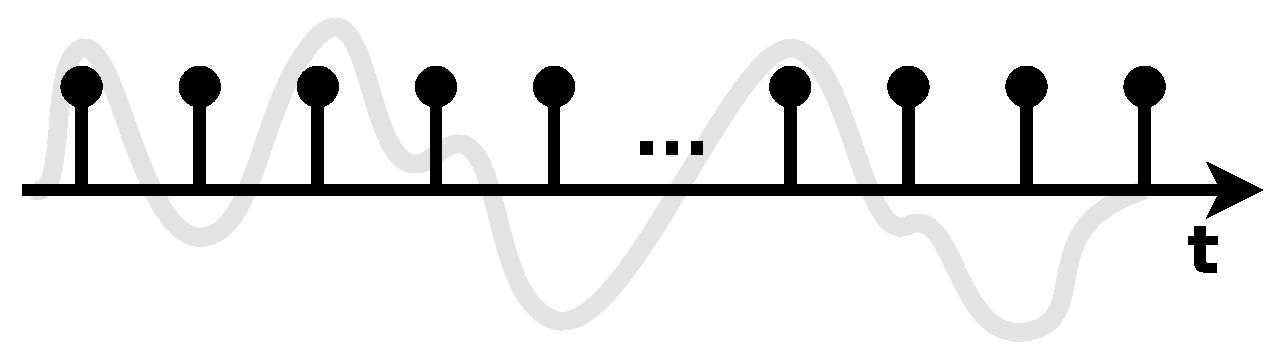
\includegraphics[width=\textwidth]{chapters/cap-musicalidade-tecnica/aspectos-metrica-a.eps}
         \caption{Simplificação da música em pulsos.}
         \label{fig:metrica:pulso}
     \end{subfigure}
     \hfill
     \begin{subfigure}[b]{0.485\textwidth}
         \centering
         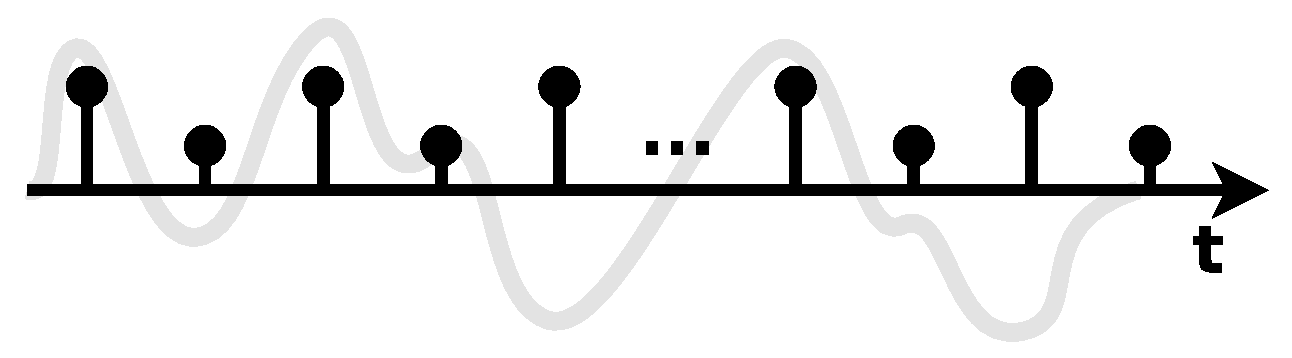
\includegraphics[width=\textwidth]{chapters/cap-musicalidade-tecnica/aspectos-metrica-b.eps}
         \caption{Simplificação da música em tempos.}
         \label{fig:metrica:tempo}
     \end{subfigure}
        \caption{Pulso vs. tempo}
        \label{fig:metricapulsotempo}
\end{figure}


Dado que estes aspectos da música que envolvem a métrica, são dos primeiros que aprendemos a reconhecer na música,
já seja de forma consciente ou inconsciente,
seu uso é considerado um estagio básico da musicalidade na nossa dança.
 
\index{Musicalidade!Bússola}
\begin{example}[Dançando com bússola:]~\\
\noindent
\begin{minipage}[t]{0.25\linewidth}
\begin{figure}[H]
  \centering
  \begin{subfigure}[t]{0.9\linewidth}
    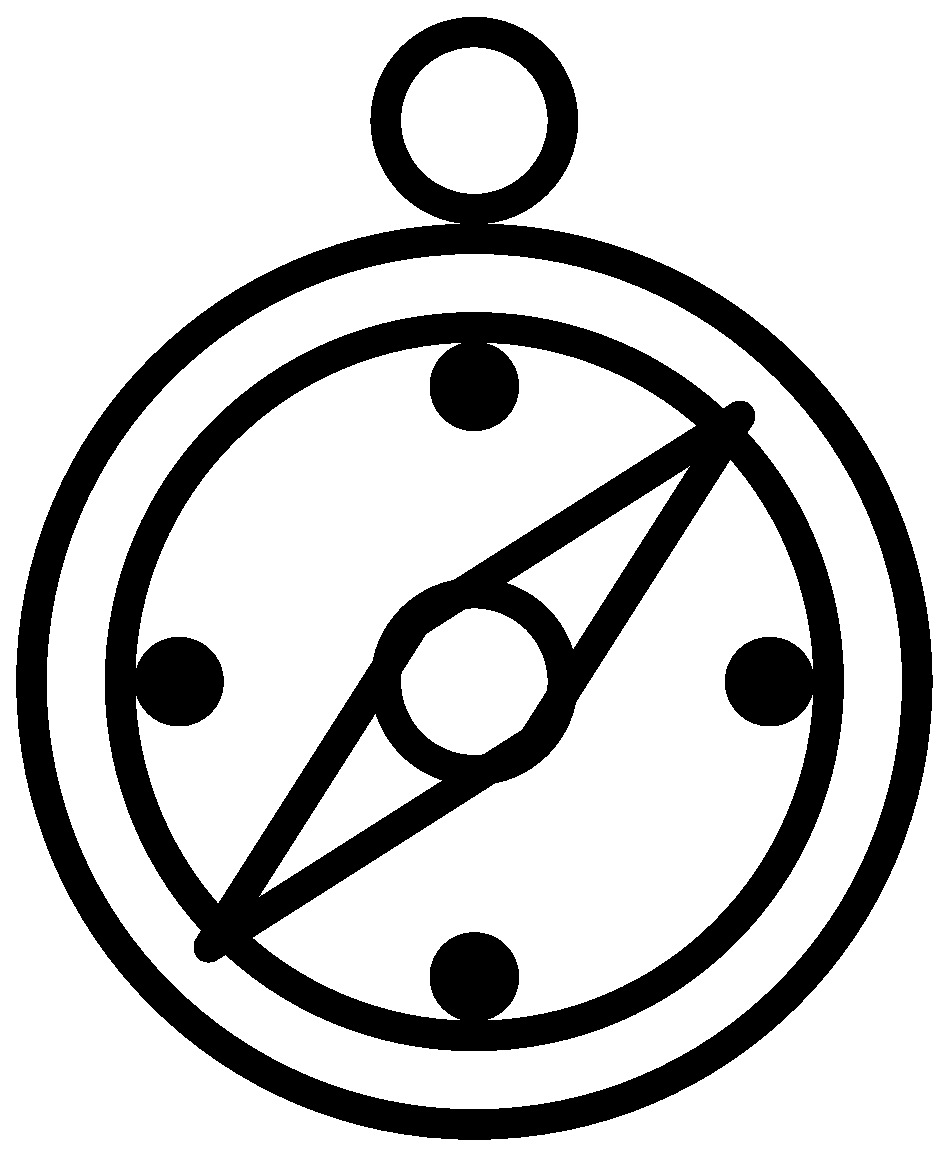
\includegraphics[width=\textwidth]{compass.eps}
  \end{subfigure}
\end{figure}
\end{minipage}
\begin{minipage}[t]{0.75\linewidth}
Se já podemos \hyperref[subsec:perceberTF1]{\textbf{reconhecer os tempos fortes}} e fracos, 
e consequentemente sabemos quando inicia um \hyperref[sec:compaso]{\textbf{compasso musical}};
então podemos usar a localização do tempo forte para orientar-nos na música,
sendo esta nossa bússola;
tendo assim una referencia para voltar a estar em sincronia com  nosso par de dança e com a música, 
quando cometemos algum erro ou quando reiniciamos nossa dança apos algum ``break''.
\end{minipage}
\end{example}


\begin{example}[Dançando executando dinâmicas:]
Quando já temos consciência dos tempos fortes e fracos,
poderíamos tomar a decisão artística de interpretar corporalmente estas percepções, 
executando os movimentos que acontecem no tempo forte com maior \hyperref[sec:musicalidadenergia]{\textbf{energia}},
e os que acontecem no tempo fraco com menor energia.
\end{example}

\begin{example}[Dançando executando ``tchic tchic tum'':]
\label{ex:dance:pulso}
Imaginemos que temos decidido executar nossos movimentos (ex: pisadas, ou movimentos de ombros, cabeça quadril, etc.),
seguindo uma distribuição de tempos ``tchic tchic tum'',
o que é equivalente a indicar que usaremos uma sequencia ``rápido rápido lento''.

Uma possível alternativa, para dançar na métrica, 
seria:
\begin{itemize} 
\item Encaixar o ``tchic tchic tum'', 
de maneira que esta distribuição de tempos encha completamente um compasso.
\item Decidindo  que o ``tum'', 
que consideramos o movimento principal da sequencia,
seja executado no tempo forte.
\end{itemize}

Seguindo estas considerações criativas,
nossa dança, 
usando a melodia ``Lamento e consolo'' (ver Figura \ref{fig:lamento-e-consolo}), 
estaria descrita como indica a Figura \ref{fig:lamentoconsolopulso1};
onde a melodia que escutamos está sendo executada por um ``bandolim'',
e as ``claves'' representam o ritmo que seguem nossos movimentos;
nesse caso foram escolhidos pisadas, como movimentos de exemplo.
É fácil perceber, nessa representação, 
como nossos movimentos usam pouco da informação que contem a melodia, 
pois a única caraterista que compartem é a métrica.
\end{example}
\begin{sidewaysfigure}
    \centering
    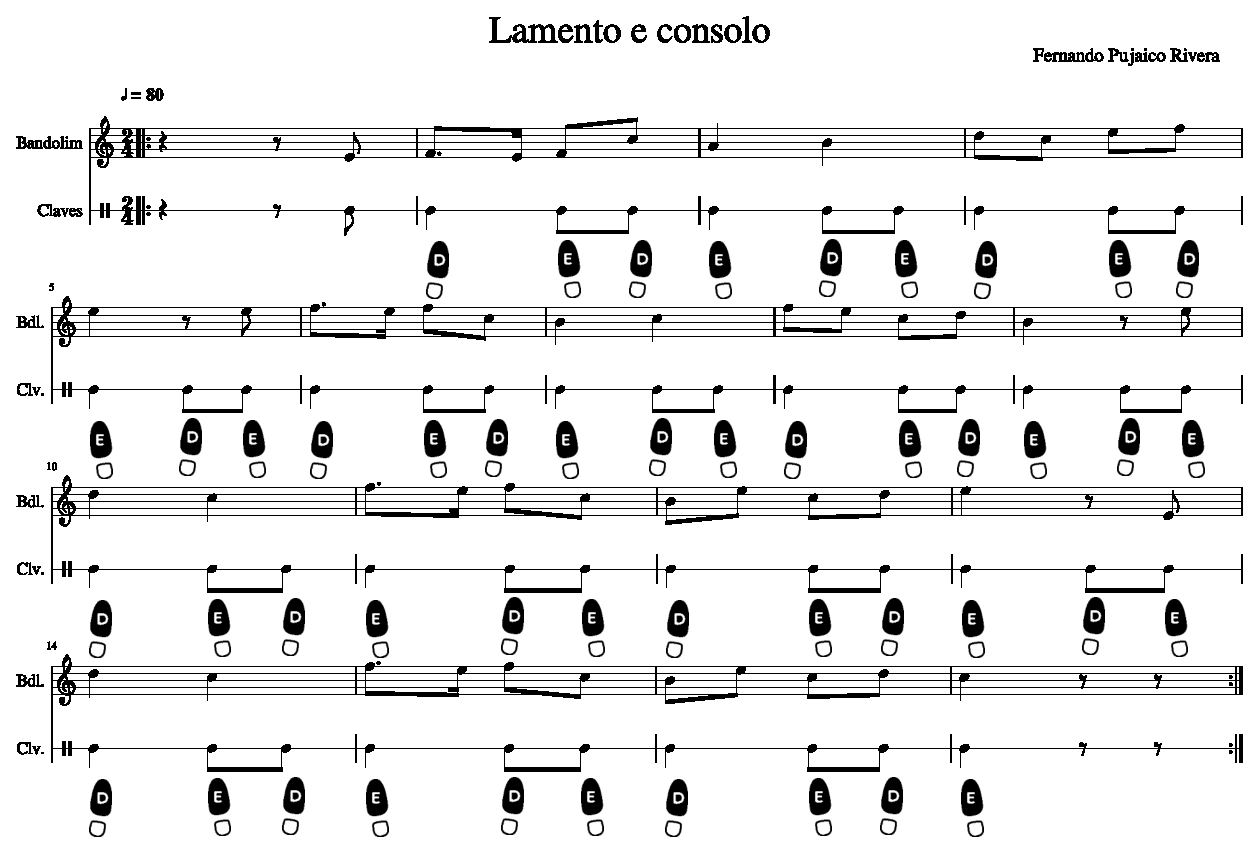
\includegraphics[width=\textwidth]{chapters/cap-musicalidade-tecnica/lamento-e-consolo-clave-pulso-1.eps}
    \caption{Música dançada na métrica.}
    \label{fig:lamentoconsolopulso1}
\end{sidewaysfigure}

\subsection{Forma evoluída de dançar na métrica ou diminuída de dançar no ritmo?}
Um caso interessante, é quando apos ter aprendido a dançar na métrica,
ganhamos consciência da música e iniciamos a prestar atenção a outros aspectos além da métrica;
percebendo detalhes como o \hyperref[sec:perceberfrases]{\textbf{final de uma frase}} rítmica, 
ou os \hyperref[sec:percepcionbreak]{\textbf{breaks}} da  música.
Nesse momento, estamos usando informação extraída das frases rítmicas, 
pelo que estritamente falando estaríamos sim,  dançando no ritmo; 
porém, dado que a maior parte do tempo dançaríamos na métrica,
 poderíamos sentir que só estamos dançando uma forma evoluída de dançar na métrica.

\begin{example}[Dançando executando ``tchic tchic tum'' e breques:]
\label{ex:ritmo:usingbreak}
Se usamos as mesmas escolhas criativas que as vistas no Exemplo \ref{ex:dance:pulso},
e além disso agregamos que usaremos as pausas, ao final das frases rítmicas,
 na melodia ``Lamento e consolo'' (ver Figura \ref{fig:lamento-e-consolo}). 
Então estaríamos movimentando-nos como indica a Figura \ref{fig:lamentoconsolopulsobreak1};
onde similarmente ao Exemplo \ref{ex:dance:pulso},
as ``claves'' representam o ritmo que seguem nossos movimentos,
neste caso exemplificado com pisadas.

É fácil perceber, nessa representação, 
como nossos movimentos usam pouco da informação que contem a melodia, 
pois as únicas carateristas que compartem, movimento e música, 
são a métrica e o acompanhamento do final de frase rítmica.
Um ponto interessante a ressaltar,
 é que se na nossa tentativa de dançar como na Figura \ref{fig:lamentoconsolopulsobreak1}, 
percebemos que temos problemas em manter, na nossa mente, a métrica durante as pausas; 
uma boa regra geral, especialmente sim somos novos na dança, 
seria realizar \hyperref[ref:pausaativa]{\textbf{pausas ativas}};
é dizer, manter a métrica da música, neste caso binária, usando alguma parte de nosso corpo.
Por exemplo, poderíamos movimentar a cabeça, os ombros, o quadril, etc.
Acompanhando mentalmente o compasso binário,
deixando um pé livre, pronto para sair no próximo tempo forte da música.
\end{example}
\begin{sidewaysfigure}
    \centering
    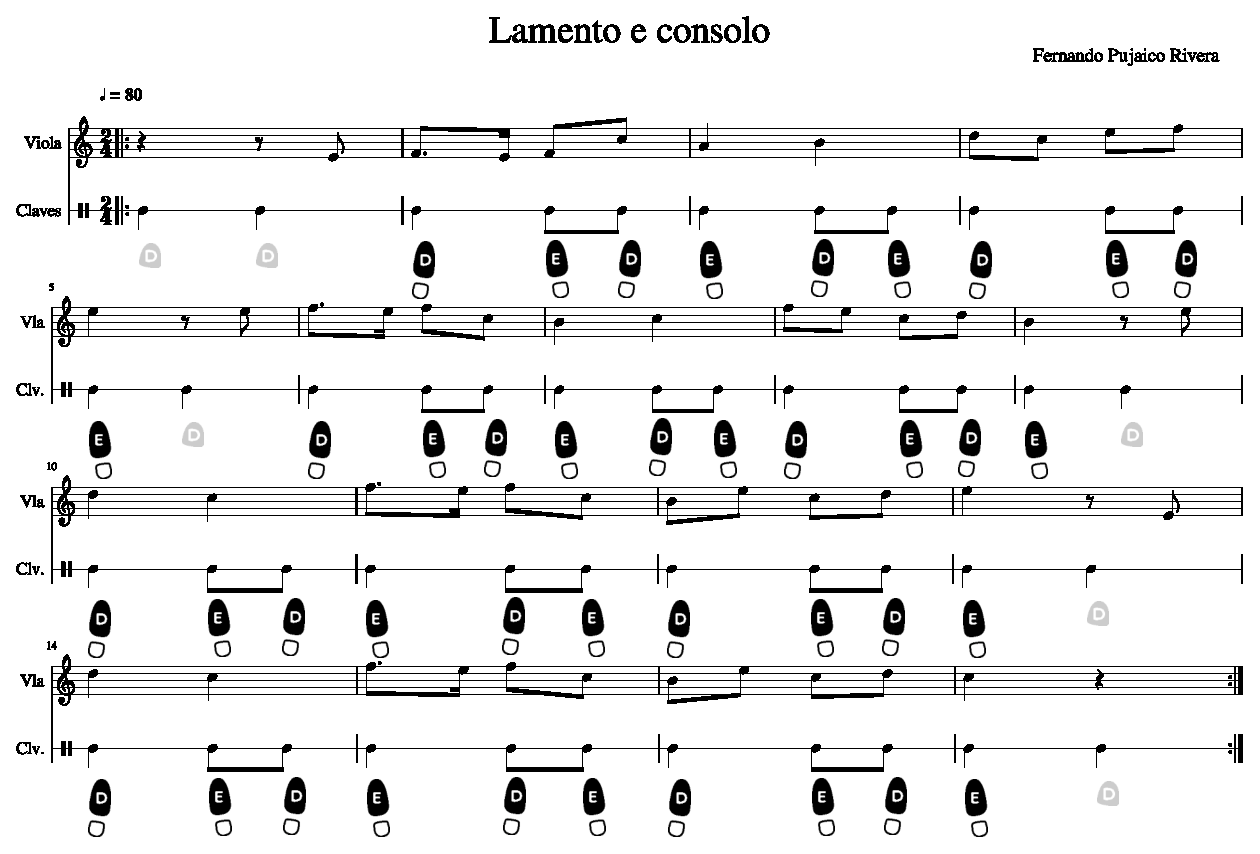
\includegraphics[width=\textwidth]{chapters/cap-musicalidade-tecnica/lamento-e-consolo-clave-pulso+break-1.eps}
    \caption{Música dançada geralmente na métrica e usando breaks.}
    \label{fig:lamentoconsolopulsobreak1}
\end{sidewaysfigure}
